\documentclass{article}
\usepackage{graphicx}
\usepackage{amsmath}
\usepackage{inputenc}
\usepackage{a4}
\usepackage{hyperref}

\begin{document}
	\title{Over Leaf}
	\author{Jayaraj Thigala}
	\date{Apri 24 ,2024}
	\maketitle
	
	\section{Introduction}
	Your introduction goes here! Simply start writing your document and use the Recompile button to
	view the updated PDF preview. Examples of commonly used commands and features are listed below,
	to help you get started.
	Once you’re familiar with the editor, you can find various project setting in the Overleaf menu,
	accessed via the button in the very top left of the editor. To view tutorials, user guides, and further
	documentation, please visit our help library, or head to our plans page to choose your plan.
	
	\section{Some examples to get Started}
	
	\subsection{ How to create Sections and Subsections }
	Simply use the section and subsection commands, as in this example document! With Overleaf, all
	the formatting and numbering is handled automatically according to the template you’ve chosen. If
	you’re using Rich Text mode, you can also create new section and subsections via the buttons in the
	editor toolbar.
	
	\subsection{How to add tables}
	Use the table and tabular environments for basic tables — see Table 1, for example. For more infor-
	mation, please see this help article on tables.
	
	\begin{table}[h]
		\centering
		\begin{tabular}{|c|c|}
			\hline
			Items & Quantity\\
			\hline
			Widgets & 42 \\
			Gadgets & 13 \\
			\hline
			
		\end{tabular}
	\end{table}
	
	\subsection{ How to includes Figures}
	First you have to upload the image file from your computer using the upload link in the file-tree menu.
	Then use the includegraphics command to include it in your document. Use the figure environment
	and the caption command to add a number and a caption to your figure. See the code for Figure 1 in
	this section for an example.
	Note that your figure will automatically be placed in the most appropriate place for it, given the
	surrounding text and taking into account other figures or tables that may be close by. You can find
	out more about adding images to your documents in this help article on including images on Overleaf.
	
	
		\begin{figure}
		\centering
		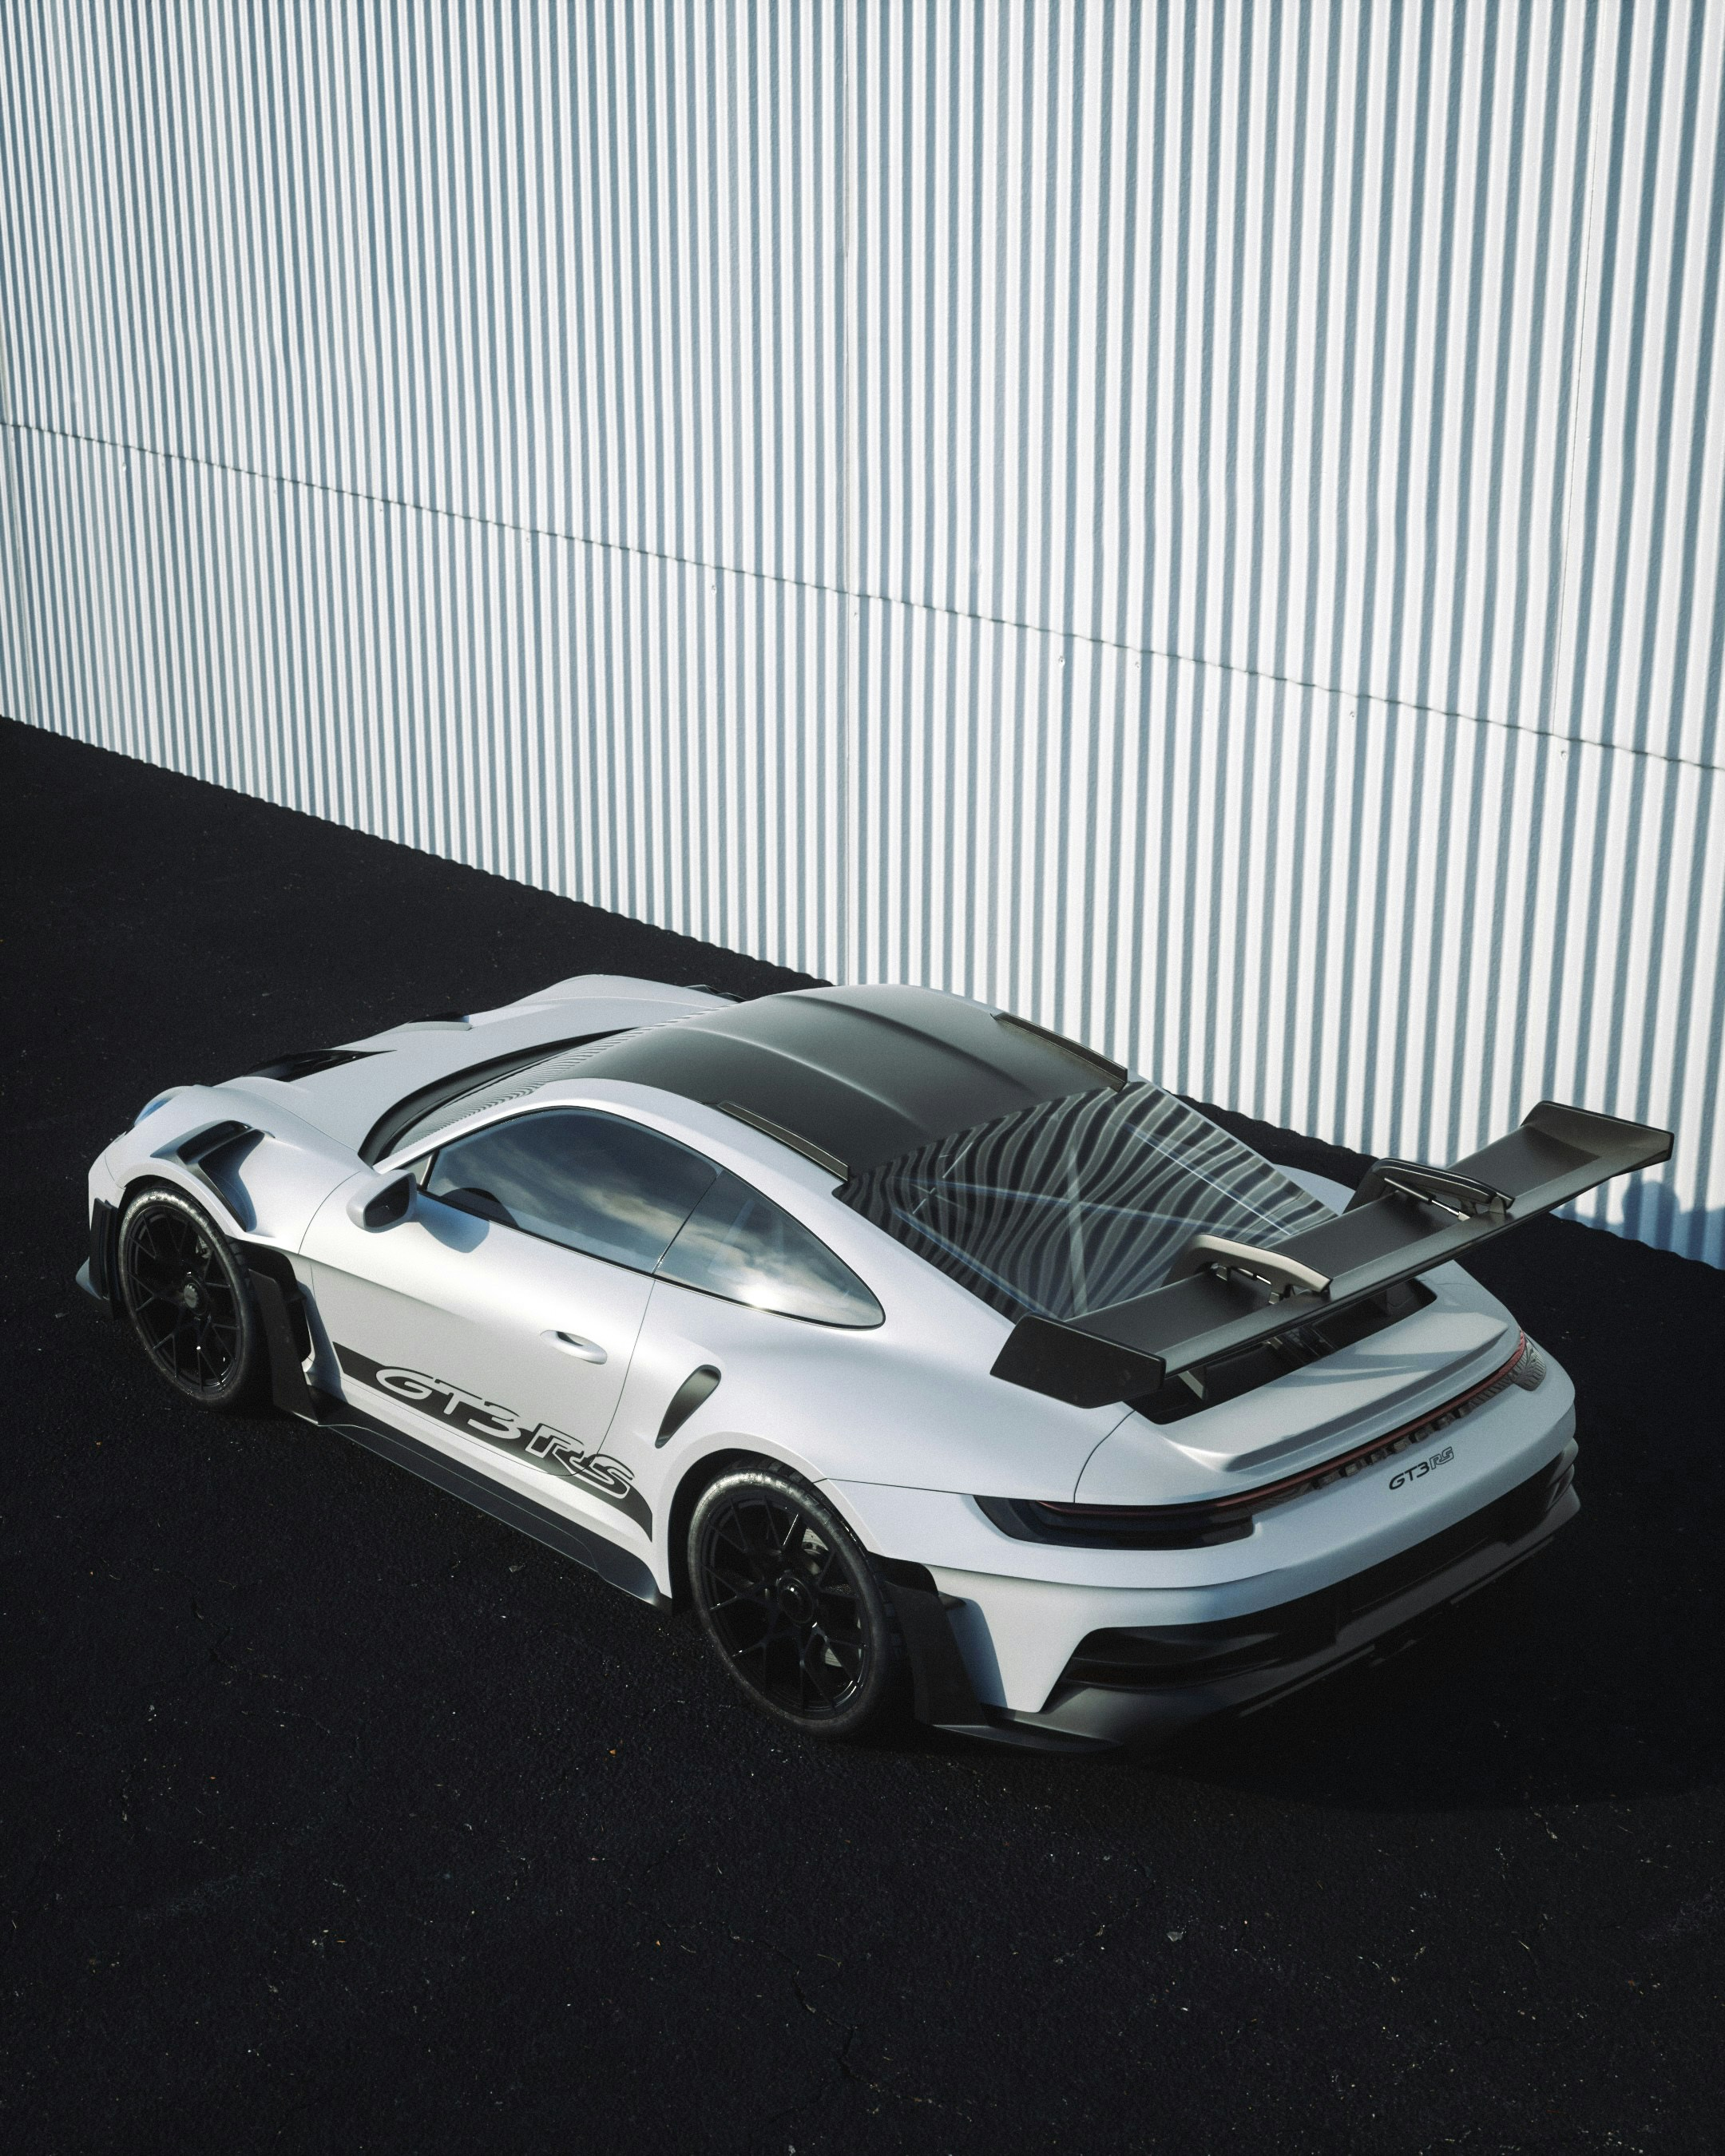
\includegraphics[width=0.5\textwidth]{image2}
		\caption{This car was uploaded via the file-tree menu. }
		\label{fig:example}
	\end{figure}
	
	\subsection{How to add Comments and Track Changes}
	
	Comments can be added to your project by highlighting some text and clicking “Add comment” in
	the top right of the editor pane. To view existing comments, click on the Review menu in the toolbar
	above. To reply to a comment, click on the Reply button in the lower right corner of the comment.
	You can close the Review pane by clicking its name on the toolbar when you’re done reviewing for the
	time being.
	Track changes are available on all our premium plans, and can be toggled on or off using the option
	at the top of the Review pane. Track changes allow you to keep track of every change made to the
	document, along with the person making the change.
	
	
	\subsection{How to Add Lists}
	
	\begin{enumerate}
		\item 
		CSE
		\item
		ECE
		\item EEE
	\end{enumerate}
$\underline{Bullet points}$
 \begin{itemize}
 	\item CSE
 	\item ECE
 \end{itemize}

\subsection{How to write Mathematics }
LATEX is great at typesetting mathematics. Let $X_{1}$ , $X_{2}$ , . . . , $X_{n}$ be a sequence of independent and
identically distributed random variables with E[$X_{i}$] = $\mu$ and Var[$X_{i}$ ] =  $\sigma$  2 < $\infty$, and let\\
\newline

$S_{n}$ = $\frac{ X_{1} + X_{2} + . . . + X_{n} }{n}$ = $\frac{1}{n}$ $\sum_{i}^{n}$ $X_{i}$ \\


denote their mean. Then as n approaches infinity, the random variables\\

	\[\sqrt{n}\] \[(S_{n} - \mu )\]

converge in distribution to a normal \[N(0,\sigma ^ 2)\]

\subsection{How to change document Language and Spelling Checks}
Overleaf supports many different languages, including multiple different languages within one document.\\

To configure the document language, simply edit the option provided to the babel package in the
preamble at the top of this example project. To learn more about the different options, please visit
this help article on international language support.
To change the spell check language, simply open the Overleaf menu at the top left of the editor
window, scroll down to the spell check setting, and adjust accordingly.

\subsection{How to add Citations and References Links }

You can simply upload a .bib file containing your BibTeX entries, created with a tool such as JabRef.
You can then cite entries from it, like this: [Gre93]. Just remember to specify a bibliography style, as
well as the filename of the .bib. You can find a video tutorial here to learn more about BibTeX.
If you have an upgraded account, you can also import your Mendeley or Zotero library directly as
a .bib file, via the upload menu in the file-tree.

\subsection{Good Luck !}
We hope you find Overleaf useful, and do take a look at our help library for more tutorials and user
guides! Please also let us know if you have any feedback using the Contact Us link at the bottom of
the Overleaf menu — or use the contact form at https://www.overleaf.com/contact.
	
\end{document}